\section{Experiments and Results}

\subsection{Lab Tank Experiments}

The system was first validated in a lab tank without the vehicle
(\autoref{f:tank}). The binocular camera was connected to a computer and 2D
relative positions of the manipulator's end effector, the target (rubber models
of sea cucumber, sea urchin and scallop with counterweight inside) are detected from its
video stream there. The processed data was transmitted to a MATLAB program
(prototype of the manipulator controlling algorithm at this early stage) to
calculate demanded air pressures to apply to the chambers of the soft
manipulator. The manipulator was fully submerged into the water and a vibration
pump was involved to simulate water flows in the real submarine environment.
With several tests, it was proved that the system has the ability to detect and
catch the seafood model with acceptable robustness. Limited by the performance
of the computer used and unoptimized algorithm, the whole process (including
detection, calculation of pressures needed with period of 1 seconds and grasp)
took about 3 minutes in average. Besides, this system could not handle targets
moving at a low speed, as well as handling static target when the system was
moving, as another result of the two factors mentioned above.

\begin{figure}[hb]
    \centering{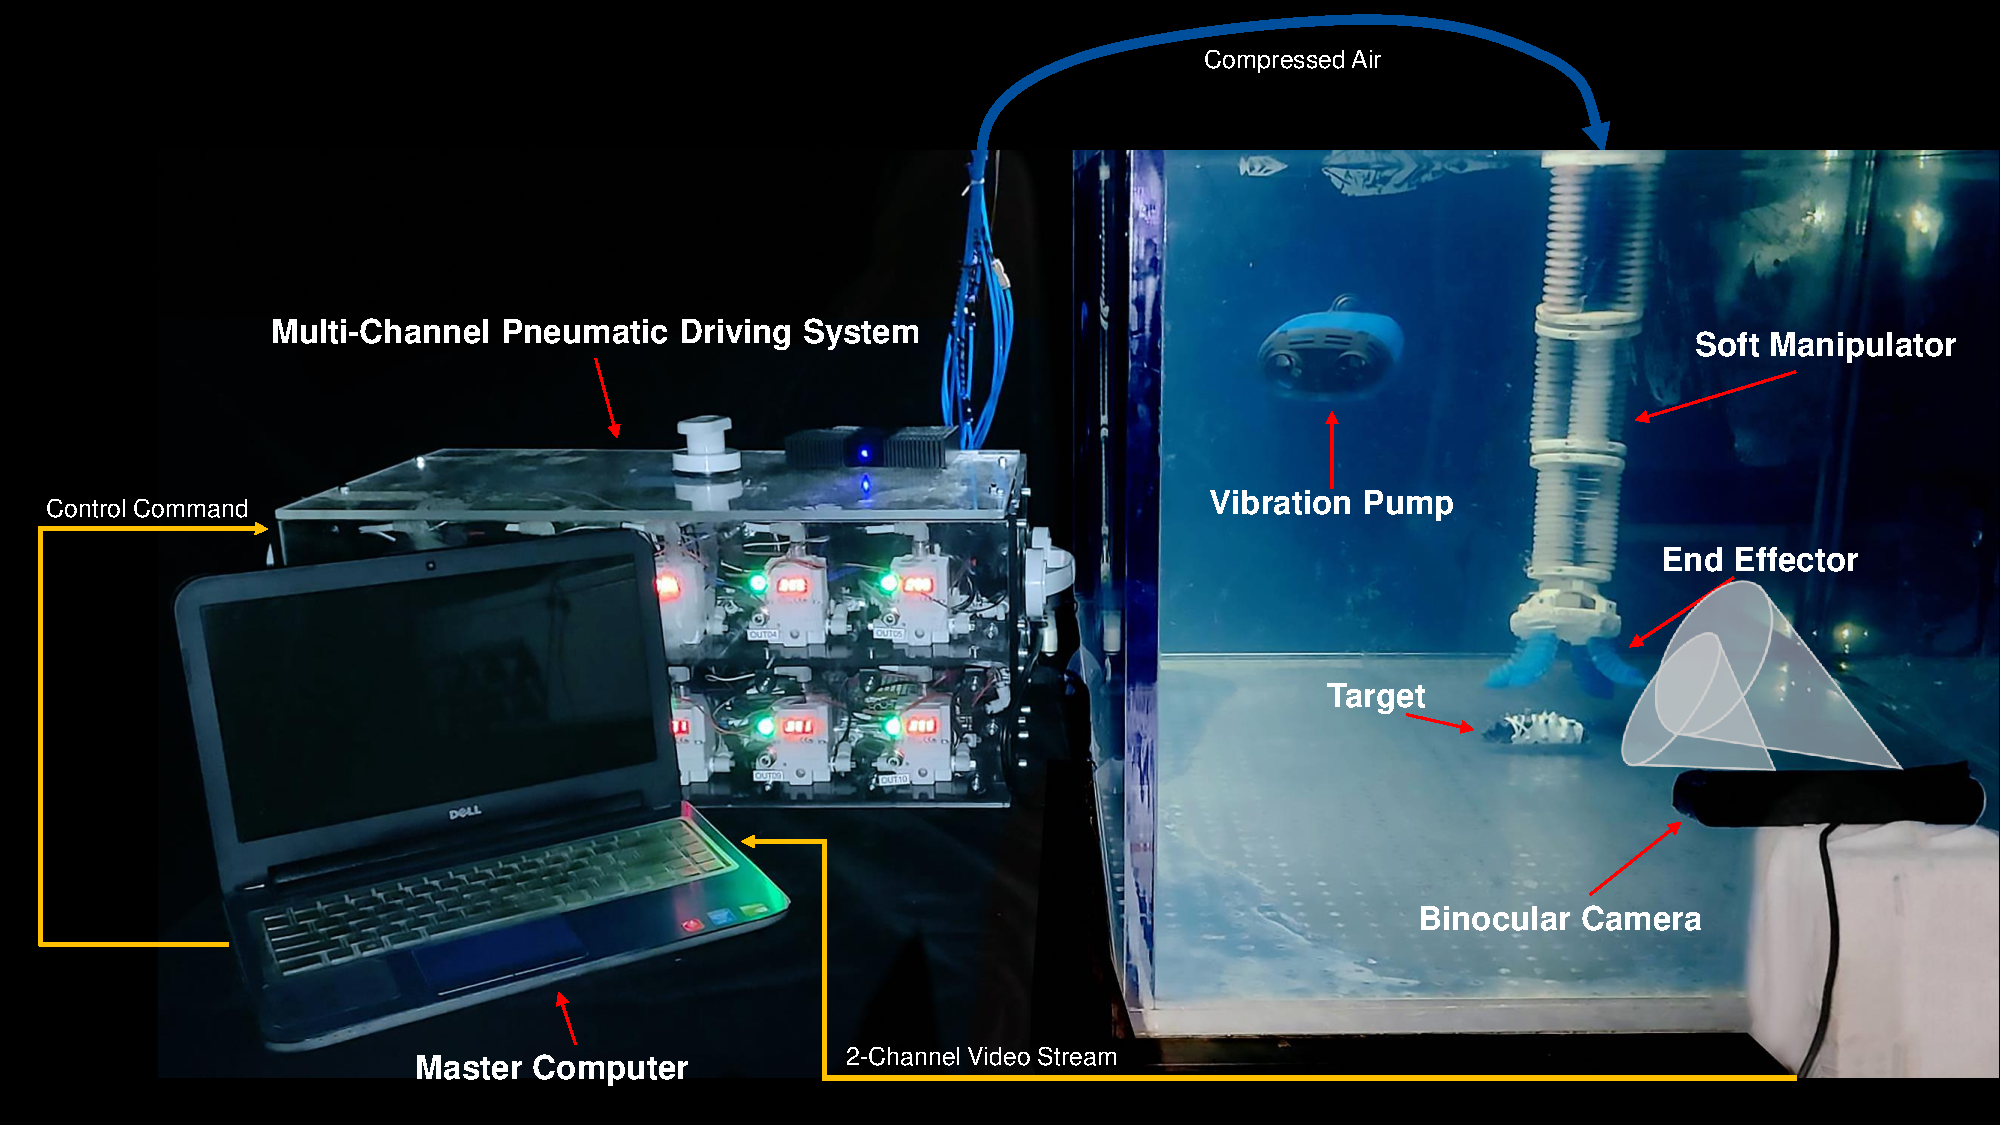
\includegraphics[width=\textwidth]{Figures/tank.pdf}}
    \caption[Early Experiment Setup at Lab Tank]{Early experiment setup at lab
    tank: the system consisted of the \gls{OBSS} soft manipulator, the pneumatic
    driving system, a computer, the \citetitle{zed} camera, a vibration pump and
    a light}\label{f:tank}
\end{figure}

\subsection{Lab Pool Experiments}

The second stage Experiments were done in a \(5m\times7m\times1.5m\) lab pool at
China Academy of Sciences Institute of Automation. The system had been developed
to as described in \autoref{s:3} at this stage. The autonomous seafood grasping
system passed both static water test and test when random moderate current were
generated by a human being at side, achieving high success rate (46 success out
of 58 attempt). \autoref{f:pool} shows snapshots of each step of how the system
successfully collected the model into its basket. How the \gls{iauv} traverse
the squared pool was shown in \autoref{f:pool} (e).

\begin{figure}[htb]
    \centering{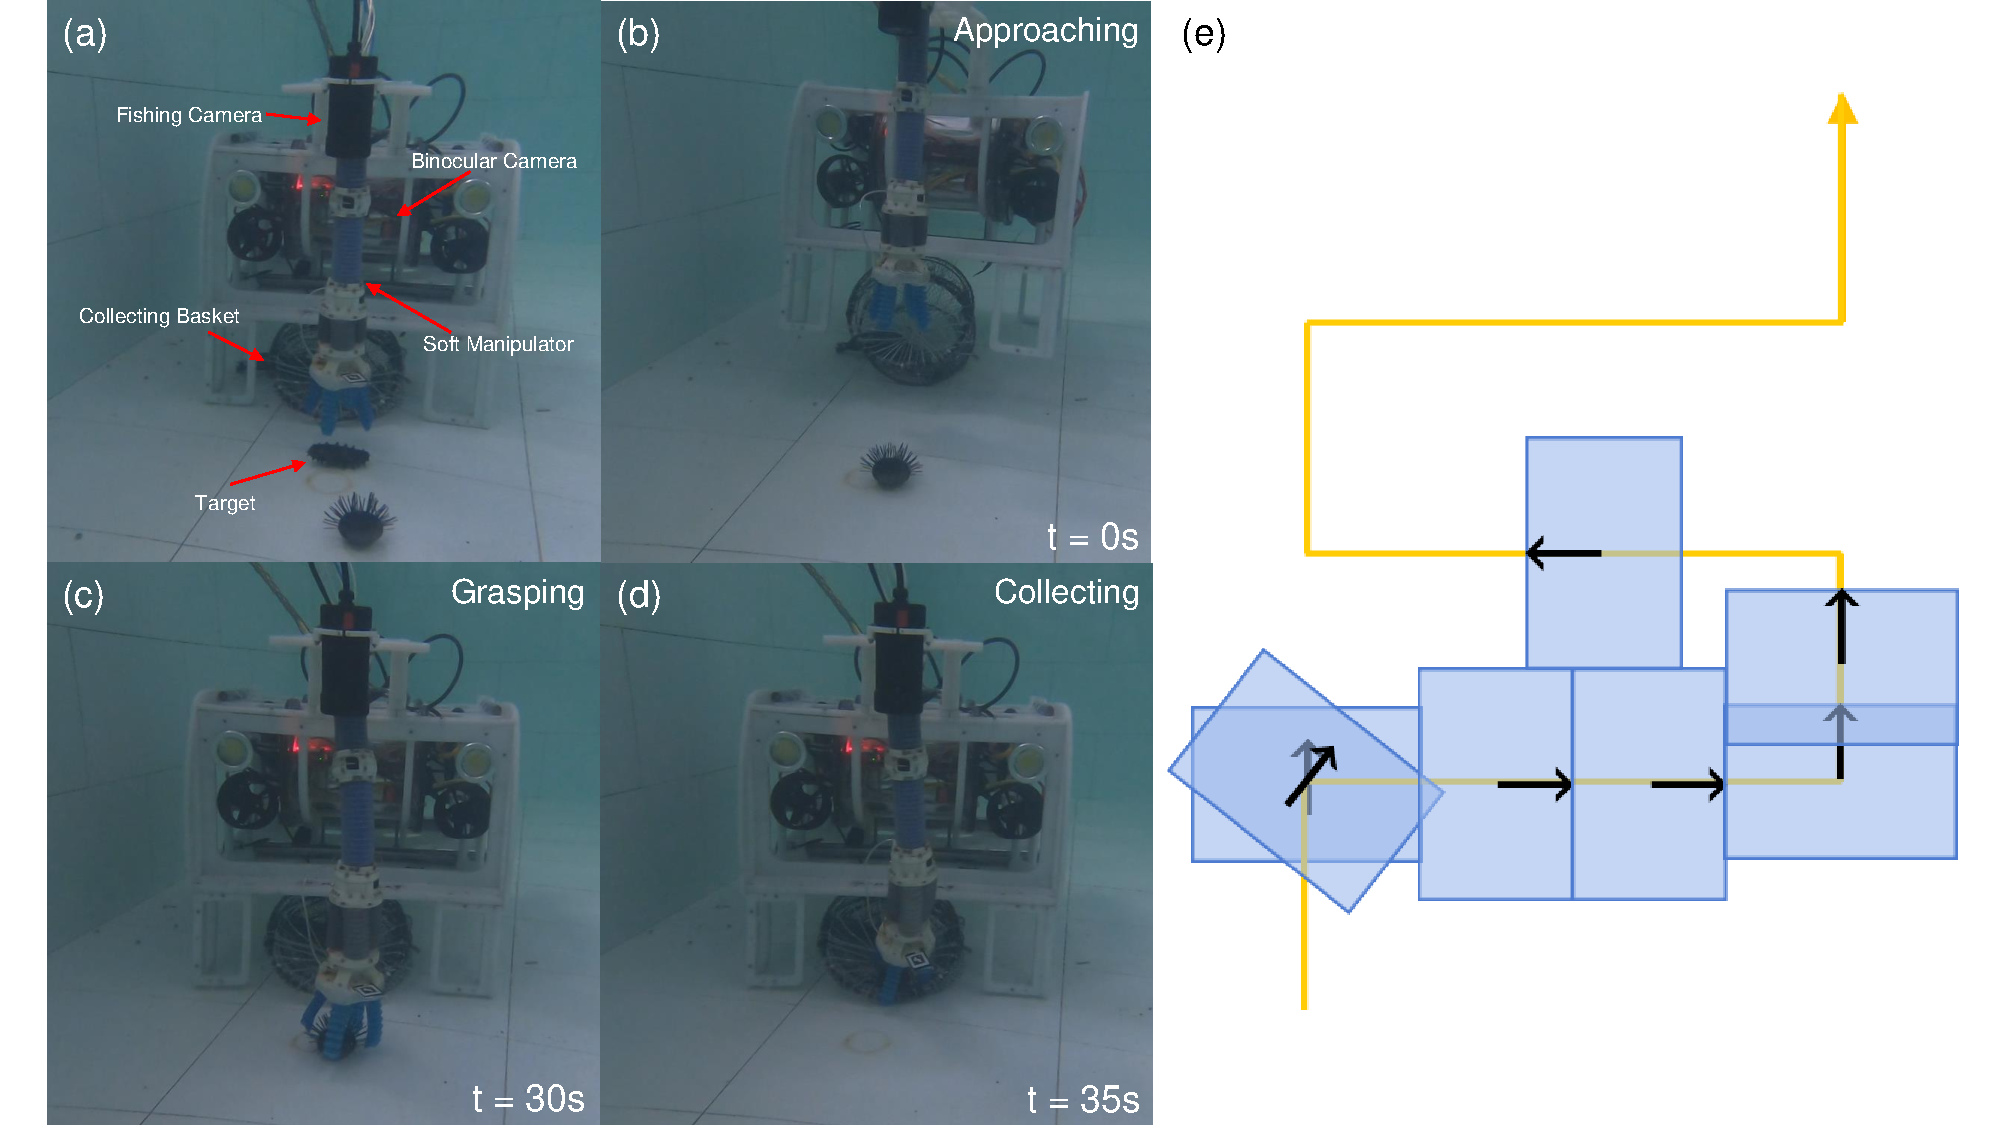
\includegraphics[width=\textwidth]{Figures/pool.pdf}}
    \caption[Grasping Procedure within the Lab Pool and Cruise Route
    Used]{Grasping procedure within the lab pool and cruise route used: (a) A
    close-up view of the \gls{iauv}. (b) The vehicle was aiming to the sea
    urchin model based on detected data automatically. (c) The vehicle was
    landed and the manipulator started to reach the model. (d) Target
    successfully collected into the basket. (e) Top view of the route used to
    traverse the pool as the blue rectangles represented the sight of the
    \gls{iauv}.}\label{f:pool}
\end{figure}

\subsection{Oceanic Experiments}

The offshore experiments were taken place at the beachside of Jinshitan in
Dalian, China. The results are shown below.

\begin{figure}[htb]
    \centering{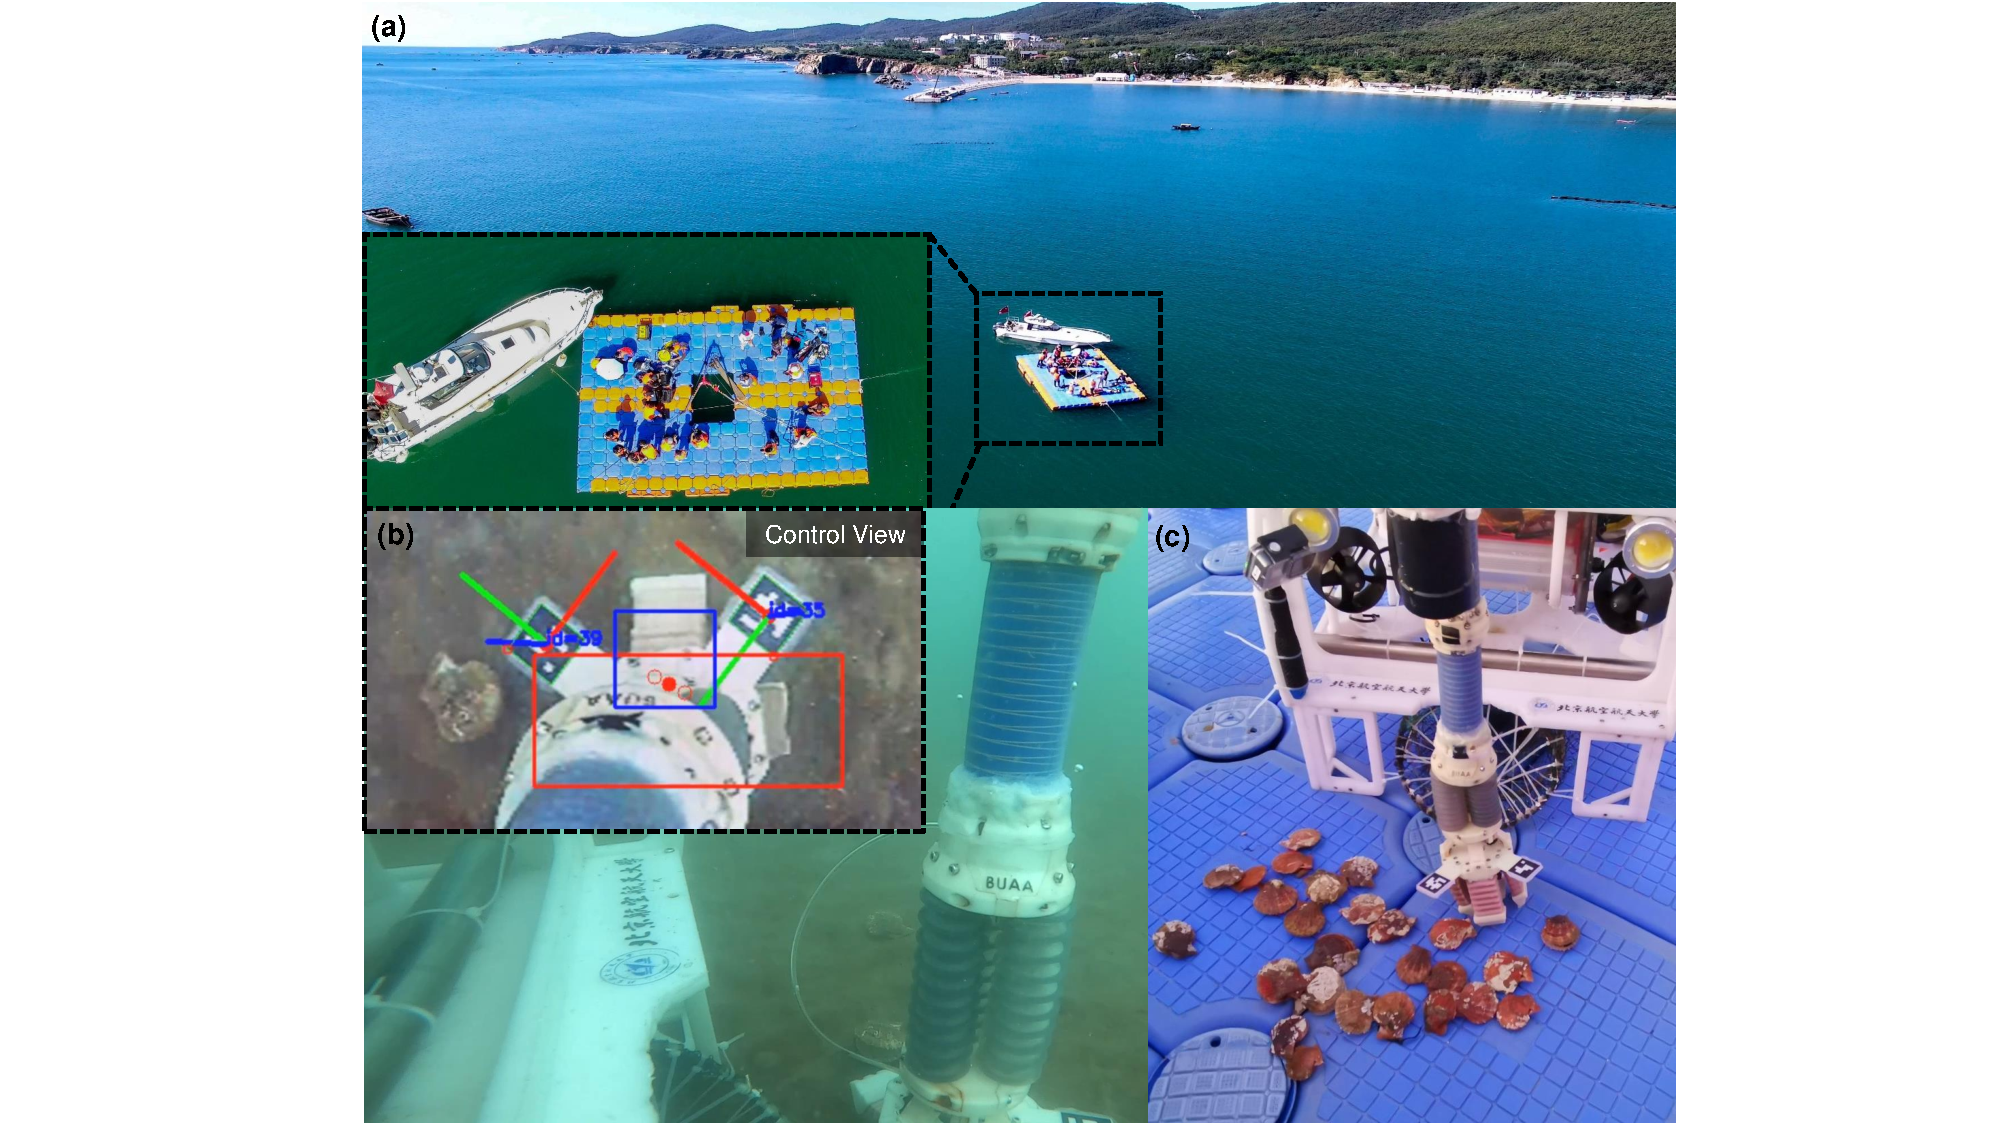
\includegraphics[width=\textwidth]{Figures/site.pdf}}
    \caption[Snapshots of site of oceanic experiments]{Snapshots of site of
    oceanic experiments: (a) The operating field of human beings (b) View from
    the master computer and fishing camera at the same time when grasping. (c)
    The harvest.}\label{f:site}
\end{figure}

\begin{figure}
    \centering{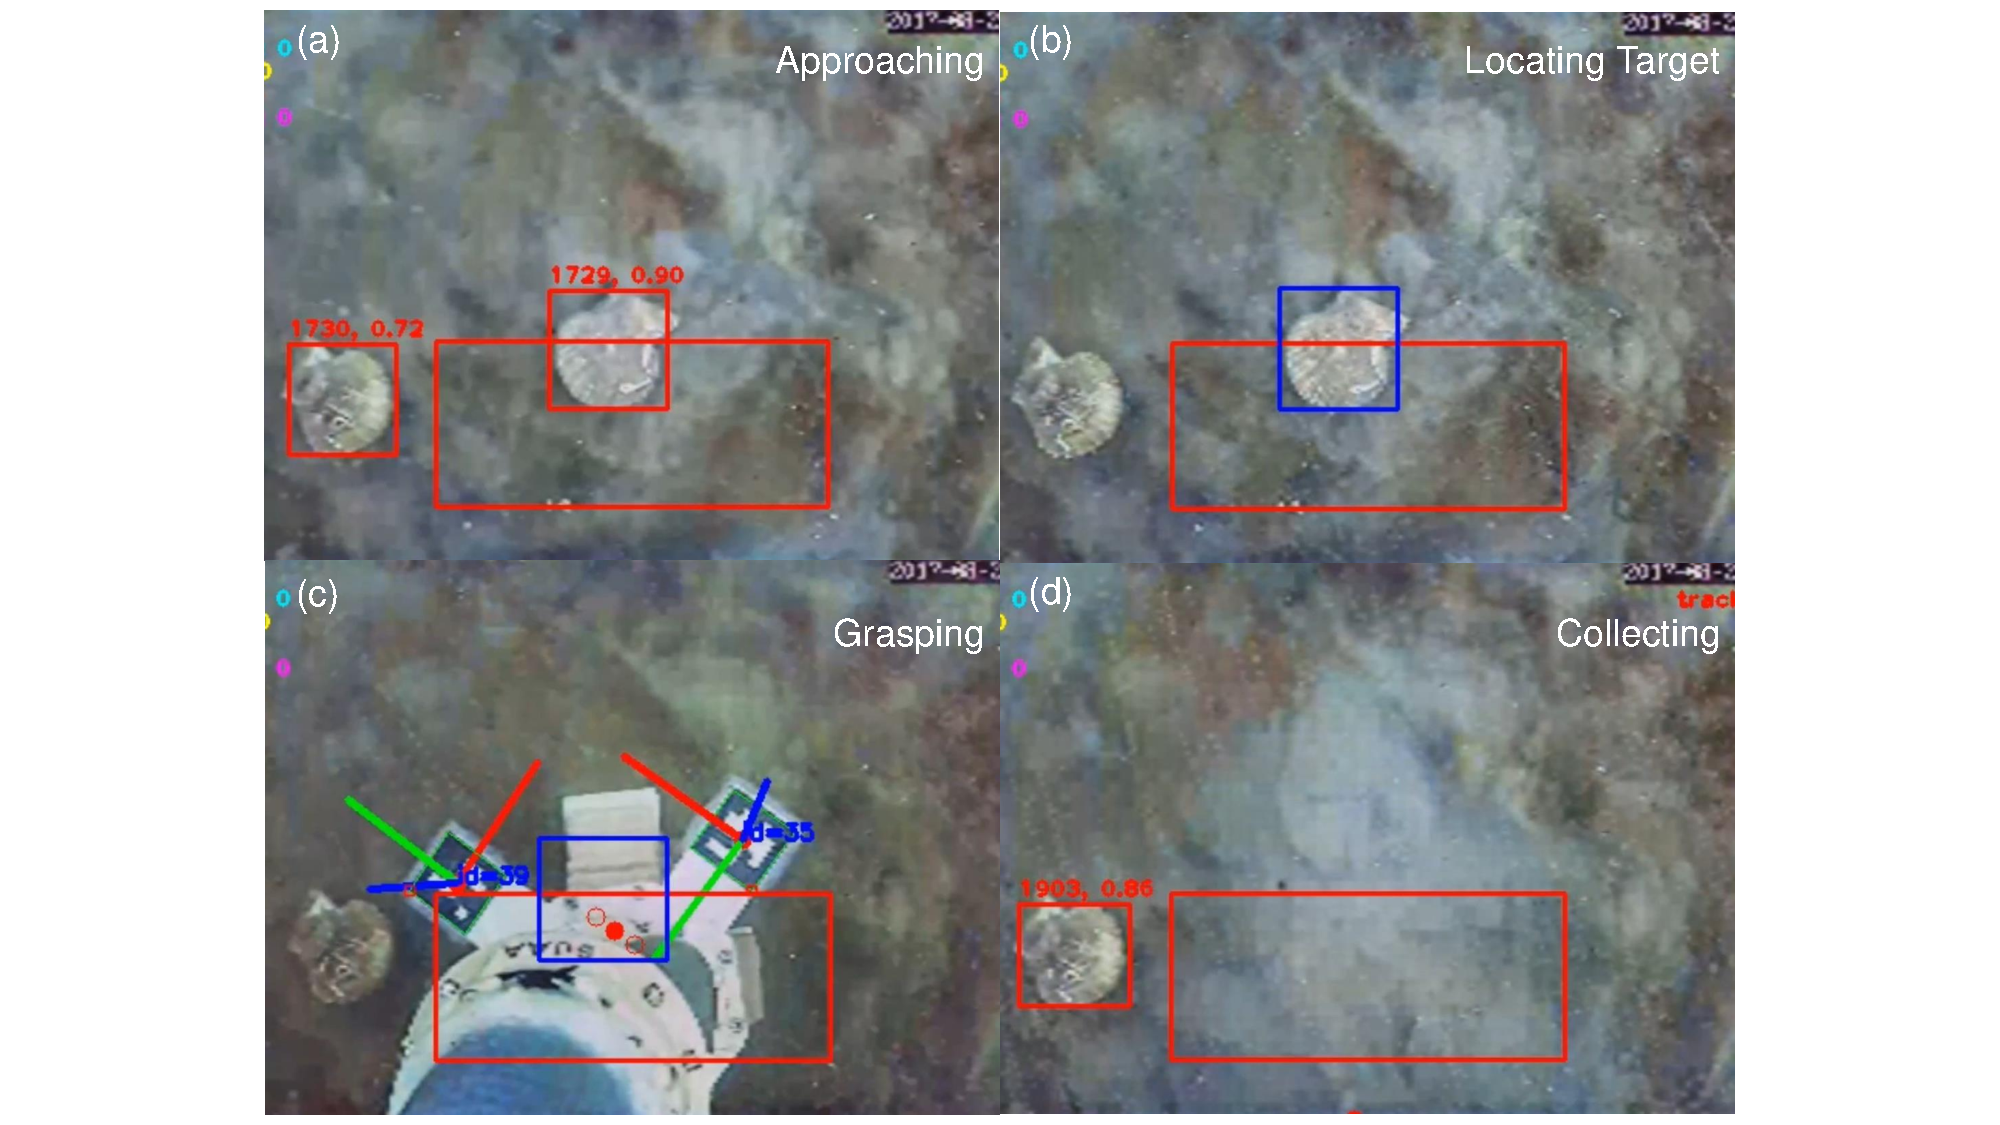
\includegraphics[width=\textwidth]{Figures/ocean.pdf}}
    \caption[Grasping Procedure Captured at Offshore Sea Bed]{Grasping procedure
        captured at offshore sea bed}\label{f:ocean}
\end{figure}